\documentclass[paper=a4paper,titlepage]{jlreq}
\usepackage[top=2cm, bottom=3cm, left=2cm, right=2cm]{geometry}
\usepackage{enumitem}
\usepackage{empheq}
\usepackage{siunitx}
\usepackage{tikz}
\usetikzlibrary{math,calc,quotes,angles}
\usepackage{tikz-3dplot}
\usepackage{xcolor}
\usepackage{wrapfig}
\usepackage{ascmac}
\usepackage{docmute}
\pagestyle{empty}
\begin{document}
\underline{氏名\hspace{330pt}得点\hspace{70pt}/25\hspace{10pt}}
\begin{itembox}[l]{問題}
    \begin{wrapfigure}[9]{r}[10pt]{0\textwidth}
        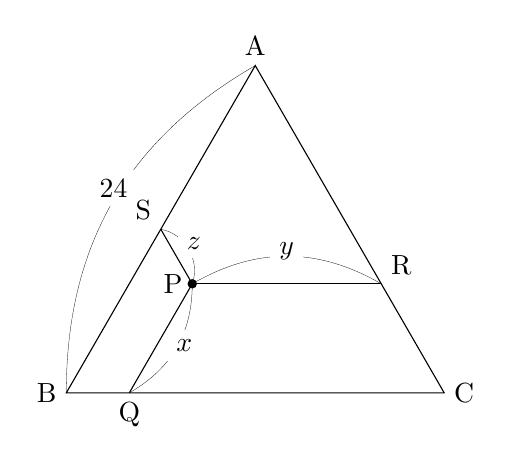
\begin{tikzpicture}[scale=0.2]
            \draw (0,0)--(24,0)--(60:24)--cycle;
            \draw (0,0) node[left]{B};
            \draw (24,0) node[right]{C};
            \draw (60:24) node[above]{A};
            \draw (8,{4*sqrt(3)}) node[left]{P};
            \draw (4,0) node[below]{Q};
            \draw (20,{4*sqrt(3)}) node[above right]{R};
            \draw (60:12) node[above left]{S};
            \draw (8,{4*sqrt(3)})--(4,0);
            \draw (8,{4*sqrt(3)})--(20,{4*sqrt(3)});
            \draw (8,{4*sqrt(3)})--(60:12);
            \fill[black](8,{4*sqrt(3)}) circle(0.3);
            \draw[ultra thin] (0,0) to [out=90,in=210] (60:24);
            \draw[ultra thin] (8,{4*sqrt(3)}) to [out=270,in=30] (4,0);
            \draw[ultra thin] (8,{4*sqrt(3)}) to [out=30,in=150] (20,{4*sqrt(3)});
            \draw[ultra thin] (8,{4*sqrt(3)}) to [out=70,in=350] (60:12);
            \draw (3,13) node[fill=white]{24};
            \draw (7.5,3) node[fill=white]{$x$};
            \draw (14,9) node[fill=white]{$y$};
            \draw (8.1,9.5) node[fill=white]{$z$};
        \end{tikzpicture}
    \end{wrapfigure}
    1辺の長さが24の正三角形の内部(周は含まない)に1点Pをとり、Pを通ってABに平行にひいた線と辺BCとの交点をQ、BCに平行な線と辺CAとの交点をR、CAに平行な線と辺ABとの交点をSとする。
    $\mathrm{PQ}=x, \mathrm{PR}=y, \mathrm{PS}=z$として、次の各問いに答えなさい。
    \\\\(1)\hspace{3pt}$x,y,z$が全て整数であるような点Pの個数を求めなさい。
    \\(2)\hspace{3pt}(1)の点を$\mathrm{P_1,P_2,...,P_n}$として、それらの点における$x,y$の値をそれぞれ$x_1,x_2,...,x_n$、
    $y_1,y_2,...,y_n$とする。このとき、$x_1+x_2+...+x_n$、$y_1+y_2+...+y_n$の値をそれぞれ求めなさい。
    \\(3)\hspace{3pt}$1\times22+2\times21+3\times20+4\times19+...+19\times4+20\times3+21\times2+22\times1$を計算しなさい。
    \\(4)\hspace{3pt}$1\times100+2\times99+3\times98+4\times97+...+97\times4+98\times3+99\times2+100\times1$を計算しなさい。
\end{itembox}
\end{document}